\section{Test sul sistema non linearizzato}

    Per fare il test del sistema di controllo sul sistema non linearizzato abbiamo implementato
    in simulink il seguente diagramma a blocchi.\\\\
    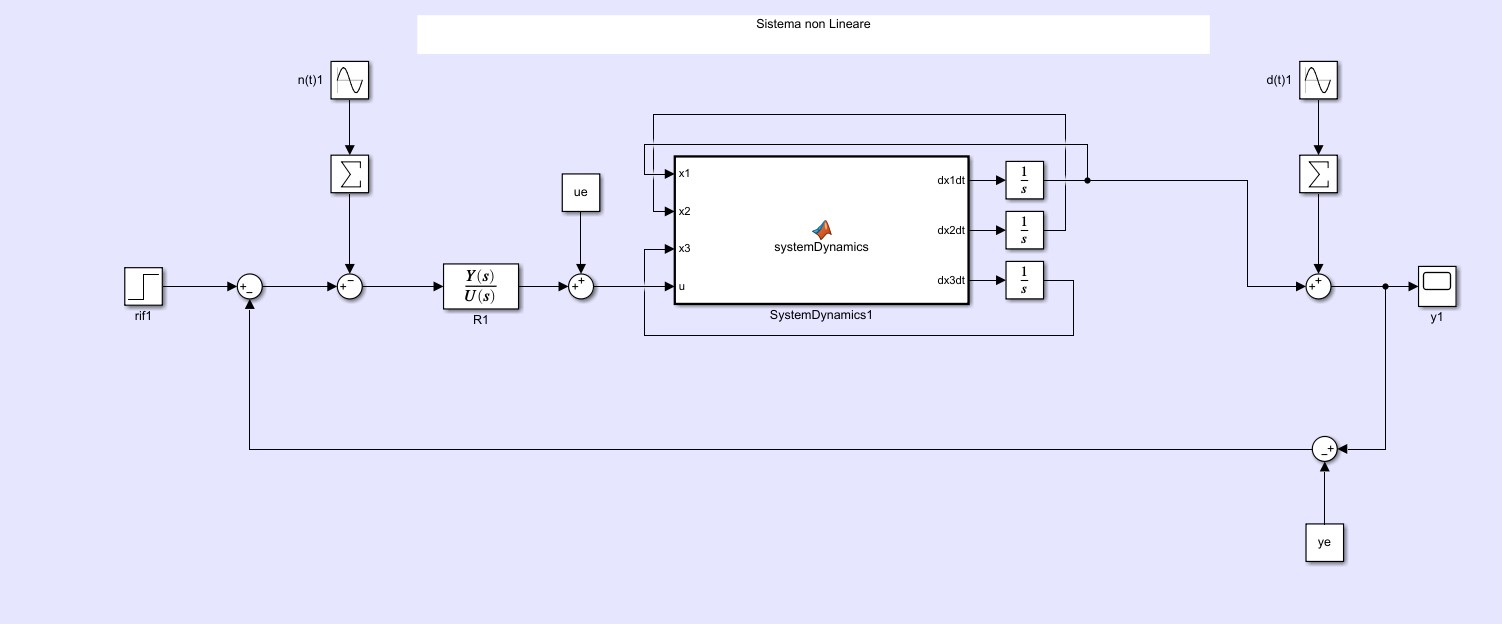
\includegraphics[scale=0.4]{immagini/diagnonlin.jpg}\\
    Nel blocco SystemDynamics abbiamo inserito il sistema non linearizzato\\\\
    \begin{adjustbox}{max width=\textwidth}
        \centering
        \begin{lstlisting}
function [dx1dt, dx2dt, dx3dt] = systemDynamics(x1, x2, x3, u)     
                    
b1=0.3;
b2=0.1; 
m=1;
k=1.5;
K_G=6.67*10^(-11);
M=5.98*10^(24);
            
dx1dt=-(2*x1*x2)/x3-(b2*x1)/m+u/(m*x3);
dx2dt=(-b1*x2+m*(k-1)*(((K_G*M)/x3^2)-x3*(x1^2)))*1/m;
dx3dt=x2;
                \end{lstlisting}
    \end{adjustbox}
    \clearpage$\\$ 
    Anche in questo caso abbiamo usato come riferimento, rumore di uscita e di misura specificati 
    nel punto precedente. \\
    Oltre a ciò abbiamo impostato come stato iniziale del sistema lo 
    stato di equilibrio (specificato mediante i blocchi integratori), ottenendo come risposta:\\\\
    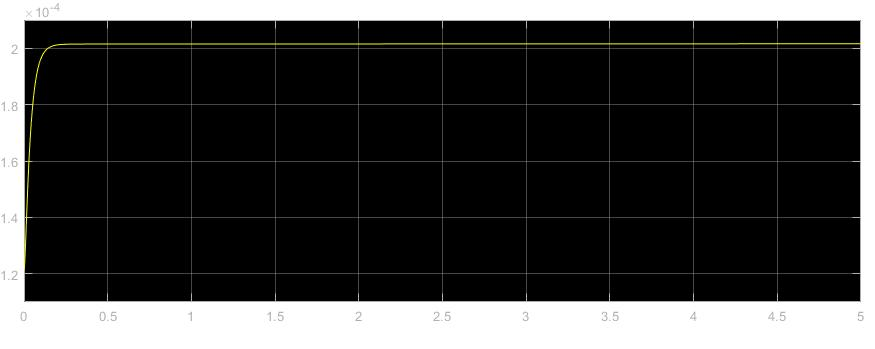
\includegraphics[scale=0.55]{immagini/rispnonlin.jpg}